\documentclass[letterpaper,12pt]{article}
\usepackage[utf8]{inputenc}
\usepackage{fullpage}
\usepackage{courier}
\usepackage[margin=0.75in]{geometry}
\usepackage{listings}
\usepackage{color}
\usepackage{graphicx}
\usepackage[width=5in]{caption}
\usepackage{hyphenat}
\usepackage[section]{placeins}
\usepackage{cmll}
\usepackage{float}
\usepackage{hyperref}

% Format a sectionless paragraph
\newcommand*\unparagraph{
	\par
	\nopagebreak
	\vskip3.25ex plus1ex minus.2ex
	\noindent
}

% define extra colors
\definecolor{dkgreen}{rgb}{0,0.6,0}
\definecolor{purple}{RGB}{159,0,197}

% define the code listing format
\lstset{
	language=C++,
	basicstyle=\footnotesize\ttfamily,
	backgroundcolor=\color{white},
	showspaces=false,
	showstringspaces=false,
	frame=none,
	tabsize=3,
	keywordstyle=\color{purple},
	commentstyle=\color{dkgreen},
	stringstyle=\color{blue},
	escapeinside={\%*}{*)}
}

% define the title/header
\title{\Large CS 1428 Honors\\Lab 8}
\author{Jared Wallace}
\date{}

\begin{document}

\maketitle

\vspace{30mm}

\section*{Overview}
Today we will be exploring Happy Prime and Non-Prime numbers. No, those are not number's that
just got back from a massage parlor, those are actually number's that meet certain
conditions. Your program today will take an input of an integer number, and will
determine whether or not that number is a Happy Prime, Happy Non-Prime,
Sad Prime or Sad Non-Prime.

\section*{Happy numbers}
To determine the happiness of a given number(positive integer only), replace the number
by the sum of the squares of its digits. Repeat this process until the number equals 1
(where it will stay), or until it loops endlessly in a cycle. Those numbers for which
this process ends in 1 are Happy numbers, whereas those that do not are Sad numbers.

Here's an example to clarify the process, using 19 as the starting value:
$$1^{2} + 9^{2} = 82$$
$$8^{2} + 2^{2} = 68$$
$$6^{2} + 8^{2} = 100$$
$$1^{2} + 0^{2} + 0^{2} = 1$$

19 is therefore Happy (and coincidently, prime). Here's another example:
$$5^{2} = 25$$
$$2^{2} + 5^{2} = 29$$
$$2^{2} + 9^{2} = 85$$
$$8^{2} + 5^{2} = 89$$
$$8^{2} + 9^{2} = 145$$
$$1^{2} + 4^{2} + 5^{2} = 42$$
$$4^{2} + 2^{2} = 20$$
$$2^{2} + 0^{2} = 4$$
$$4^{2} = 16$$
$$1^{2} + 6^{2} = \textcolor{red}{37}$$
$$3^{2} + 7^{2} = 30$$
$$3^{2} + 0^{2} = 9$$
$$9^{2} = 81$$
$$8^{2} + 1^{2} = 65$$
$$6^{2} + 5^{2} = 61$$
$$6^{2} + 1^{2} = \textcolor{red}{37}$$

\section*{Program}
This program will test your knowledge of sorting and searching. The program
should use functions for all major processing.
You will need to keep track of all the sums you calculate in an array(named \emph{cycle}).
This is so that you can detect the presence of a loop (like the second example). The array 
can be as large as 20 elements so long as you don’t exceed the maximum
value of an integer.

The algorithm to find a happy number works like this:
\begin{enumerate}
    \item Add the squares of the digits of the number together.
    \item Attempt to add the numbers to the array.
        \begin{itemize}
            \item If the number you wish to add does not exist in the array, and the array size
                has not yet reached 20, add the number to the end of the array and re-sort it.
            \item If the number \emph{does} exist in the array, you have detected a loop and, well,
                you know what to do.
        \end{itemize}
    \item Rinse, Repeat
\end{enumerate}

You should have a total of five functions in your program:
\begin{enumerate}
    \item \textbf{bool IsPrime} - This function will check to see whether the number is Prime. (Feel free to use your previous lab code for this)
    \item \textbf{bool IsHappy} - This function will check to see whether the number is Happy.
    \item \textbf{bool AddToCycle} - This function attempts to add the latest sum to the array.
       If the number already exists within the array, the function returns false.
       If the number doesn’t exist in the array it adds it, sorts the array, and returns true.
    \item \textbf{bool CycleContains} - Checks to see whether a number is in the array using a linear search.
    \item \textbf{void SelectionSort} Sorts the array using the selection sort algorithm.
\end{enumerate}

\section*{Grading}
Your implementation of this program is worth 100 points. For an extra 10 bonus points,
you may implement a binary search method in place of the default selection sort (rename your function in this case)


\section*{Deliverables}
Hard copy of the source code you wrote (happy.cpp). Soft copy (upload to homework upload) of
your source code. You may, at your discretion, use Git for version control -- it is not required.

% Comic at the bottom
\begin{figure}[ht!]
	\centering
	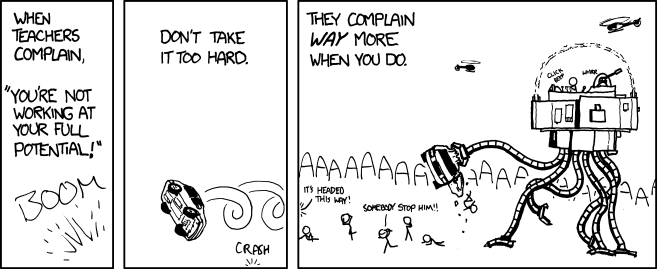
\includegraphics[width=6in]{potential.png}
    \caption*{The bunch of disadvantaged kids I was tutoring became too good at writing, and their essays were forcing me to confront painful existential questions, so I started trying to turn them on to drugs and crime instead.}
\end{figure}
\end{document}
